\section{Physics Triggers}
\label{sec:physics_triggers}

\subsection{Electron Trigger}
\label{sec:electron_trigger}

The electron trigger is designed to select inclusive electron scattering from the CLAS12 targets:
\begin{equation}
e(p,n,A) \to e' X.
\label{eqn:electron}
\end{equation}
\noindent
The trigger selects events with at least one scattered electron detected by the forward detectors. The High
Threshold Cherenkov Counter (HTCC), Pre-shower Calorimeter (PCAL),  Electromagnetic Calorimeter (EC), and
Drift Chambers (DCs) participate in the generation of the trigger decision. Searching for the electrons is
performed in all six CLAS12 Forward Detector sectors in parallel. The final electron trigger is  a simple ``OR''
of the six sector trigger signals.

The HTCC discriminates electrons from other charged particles. This detector must be calibrated in terms of
the number of photoelectrons before the start of any experiment. The HTCC trigger logic  searches for clusters
and calculates the total number of  photoelectrons  detected by the HTCC. The cluster may include up to four
PMT signals that collect the Cherenkov light from the adjacent mirrors as described in Section ~\ref{sec:HTCC}.
The minimum number of  photoelectrons in the cluster  is one of the main electron trigger parameters. Usually
this threshold is set to 1-2 photoelectrons depending on the experiment requirements.

The PCAL and EC calorimeters are designed to detect photons and electrons as described in
Section~\ref{sec:ECAL}. A high energy deposition in the calorimeters is a signature of electron detection, and
is one of the electron trigger parameters. The PCAL and EC detectors must be calibrated before the start of
any experiment in terms of energy deposition measured in MeV. The electron trigger uses cuts on the cluster
energy in the PCAL ($E_{PCAL}$) and EC ($E_{EC}$) separately, and cuts on the total energy deposition in both
detectors $E_{Total}=E_{PCAL}+E_{EC}$. These cuts depend on the beam energy and the experiment requirements,
and usually lie in the range from 150-300~MeV (corresponding to a minimum electron energy from
600-1200~MeV when accounting for the sampling fraction of the ECAL~\cite{ec-ref}) for the energy sum
$E_{Total}$.

Geometrical matching between the HTCC signal and the position of the shower in the PCAL calorimeter helps to
suppress random coincidences between the two detectors. The trigger firmware uses an HTCC-PCAL look-up
table to make a proper event selection.

The track reconstruction in the DC system at the trigger level is very useful for the further suppression of
accidental background, as described in Section ~\ref{sec:DC}. The trigger decision requires at least 3 layers
in every superlayer and at least 5 superlayers in every road, which is a standard setting for all triggers where
the DC-based component is used. The geometrical matching between track candidates and hits in the PCAL and
EC detectors is used to strengthen the trigger performance in terms of event purity.

\begin{figure}[!htb]
 	\centering
  	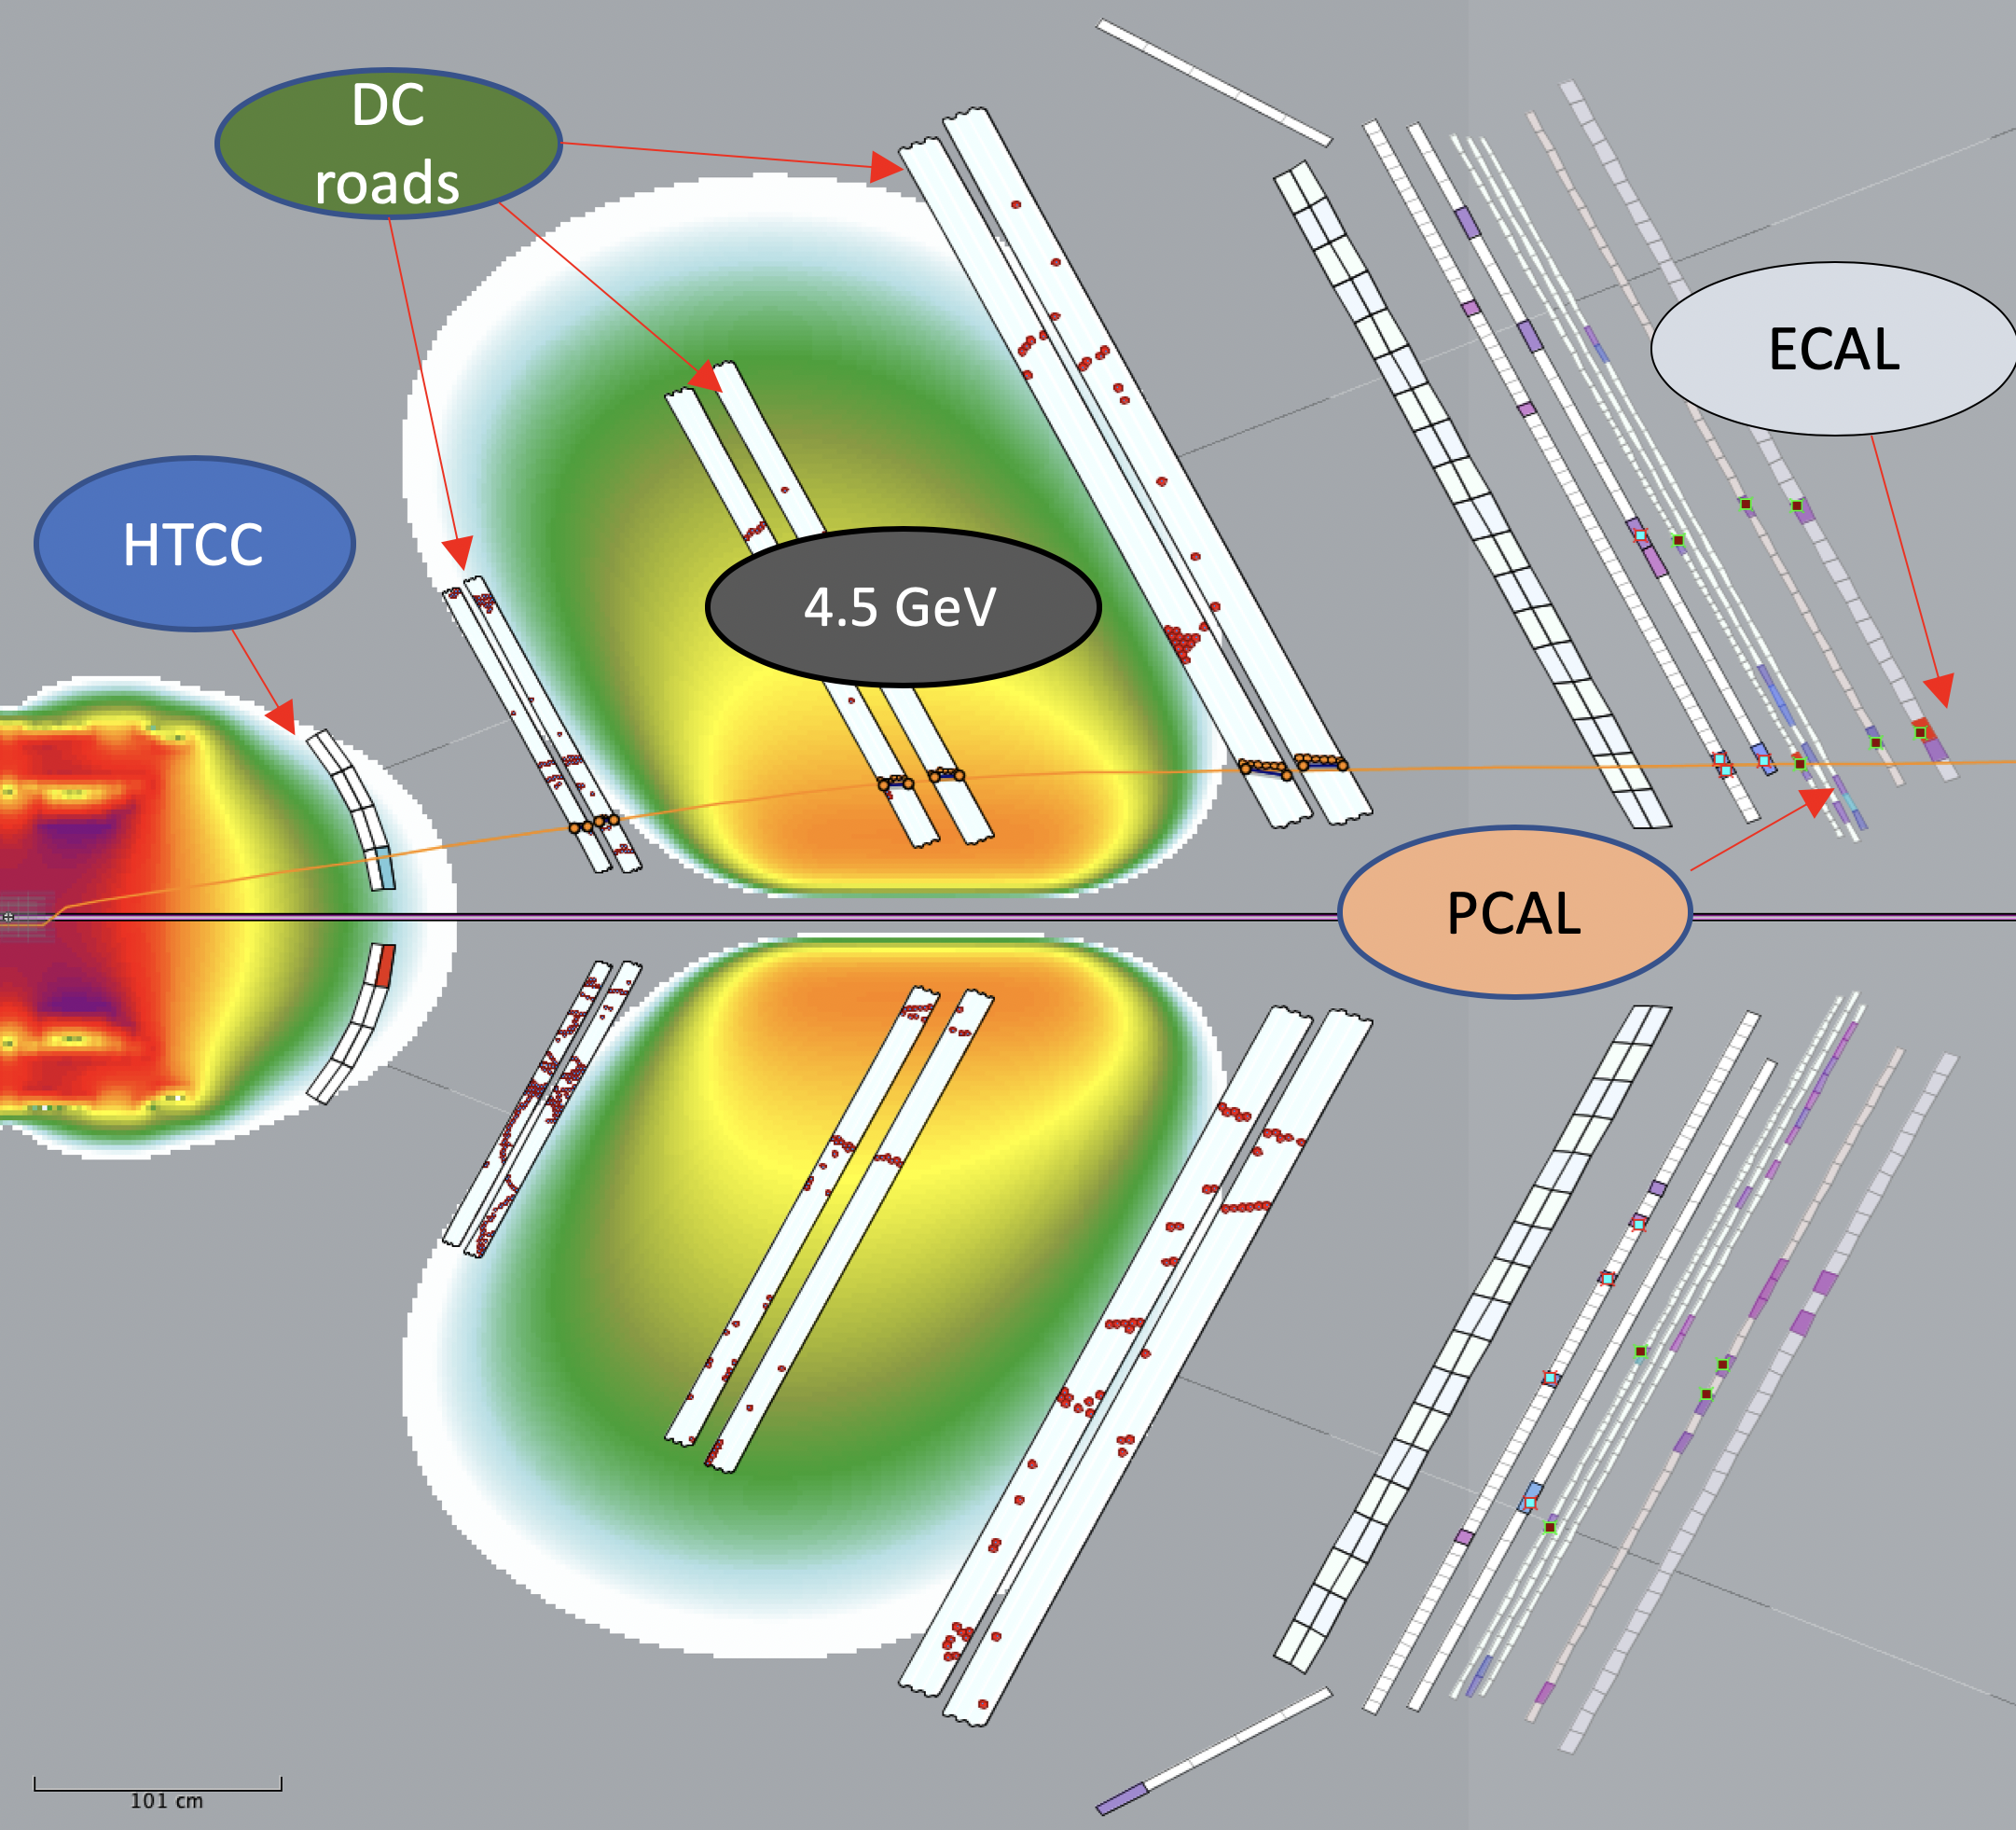
\includegraphics[width=0.95\columnwidth,keepaspectratio]{img/Electron_trigger.png}
 	\caption{Cut view from the CLAS12 event display showing an event selected by the electron trigger. The
          trigger detectors HTCC, DC, PCAL, and ECAL are indicated. The reconstructed electron momentum is
          4.5~GeV.}
	\label{fig:electron}
\end{figure}

The electron trigger configuration may be represented by the formula:
\begin{align} 
\label{eq:em_trg_formula}
\begin{split}
 & HTCC_i(N_{phe}{>}N^{HTCC}_{min})\times\\
 & [E_{PCAL}{>}E^{PCAL}_{min}) \times E_{Total}{>}E^{Total}_{min})\times  DC]_i
 \end{split}
\end{align}
\noindent
where index $i$ is the CLAS12 sector number and $N_{phe}$ is the number of photoelectrons detected by the
HTCC in a defined cluster. $N^{HTCC}_{min}$,  $E^{PCAL}_{min}$, $ E^{Total}_{min}$ are trigger parameters, and
$DC$ means that a track was reconstructed by the $DC$-system. The space correlations between all detectors
and coordinates of the track are implemented as well. As an example, the event display with a 4.5~GeV electron
selected by the trigger is shown in Fig.~\ref{fig:electron}.

\subsection{Photoproduction Trigger}
\label{sec:photoproduction_trigger}

The photoproduction trigger is designed to select events where a scattered electron is detected by the
Forward Tagger in the polar angular range from 2$^\circ$ to 5$^\circ$. Strictly speaking it is not a
photoproduction process but electron scattering with low four-momentum transfer
$Q^2=4E_{beam}E'\sin^2\theta/2$. The trigger logic continuously searches for clusters in the FT calorimeter
(FT-Cal) from an electromagnetic shower, and calculates the shower energy and space coordinates. The cluster
energy is the sum of all  crystal energies within a 3$\times$3 spatial array that meet the time-matching
constraints. Once the clustering algorithm  has identified a cluster, the corresponding data is reported to the
next trigger stage. This includes the time stamp, the energy, and the spatial coordinates (center of the seed
crystal). The cluster energy is not corrected for shower leakage effects at this stage. Finally, the trigger
processor makes the trigger decision by applying further cuts to the clusters.

The trigger selection is based on lower and upper energy limits and the number of hits in the cluster. The trigger
may also select events with a specified number of clusters detected by the calorimeter. The coincidence with
the two-plane scintillating hodoscope FT-Hodo, located in front of the calorimeter, serves to discriminate
charged particles from high-energy photons. The geometry matching between FT cluster and FT-Hodo hit
helps to suppress background coming from photons.  The trigger logics also provides  the possibility to select
reactions with an electron and several photons in the final state, for example
$$
ep\to e'\gamma\gamma X.
$$
\noindent
The display of two events with  one and two clusters in the FT-Cal, selected by the FT trigger is shown in
Fig.~\ref{fig:FT_trigger}.

The Trigger System may use the  information from the CLAS12 Forward and Central Detectors to select
events with several charged or neutral particles in coincidence with the electron in the FT-Cal. The trigger
detector composition depends on the reaction under study. 

Charged particles in the forward detectors are selected by a coincidence between the FTOF, PCAL, and EC
with tracks reconstructed by the DC system. Space correlations between all trigger detectors are required,
including coordinates of tracks crossing the detector planes. Hit matching along the track is an important
part of the background reduction at the trigger level. The cuts on the energy depositions in the trigger
detectors are used to select charged and neutral particles. 

 \begin{figure}[!htb]
 	\centering
  	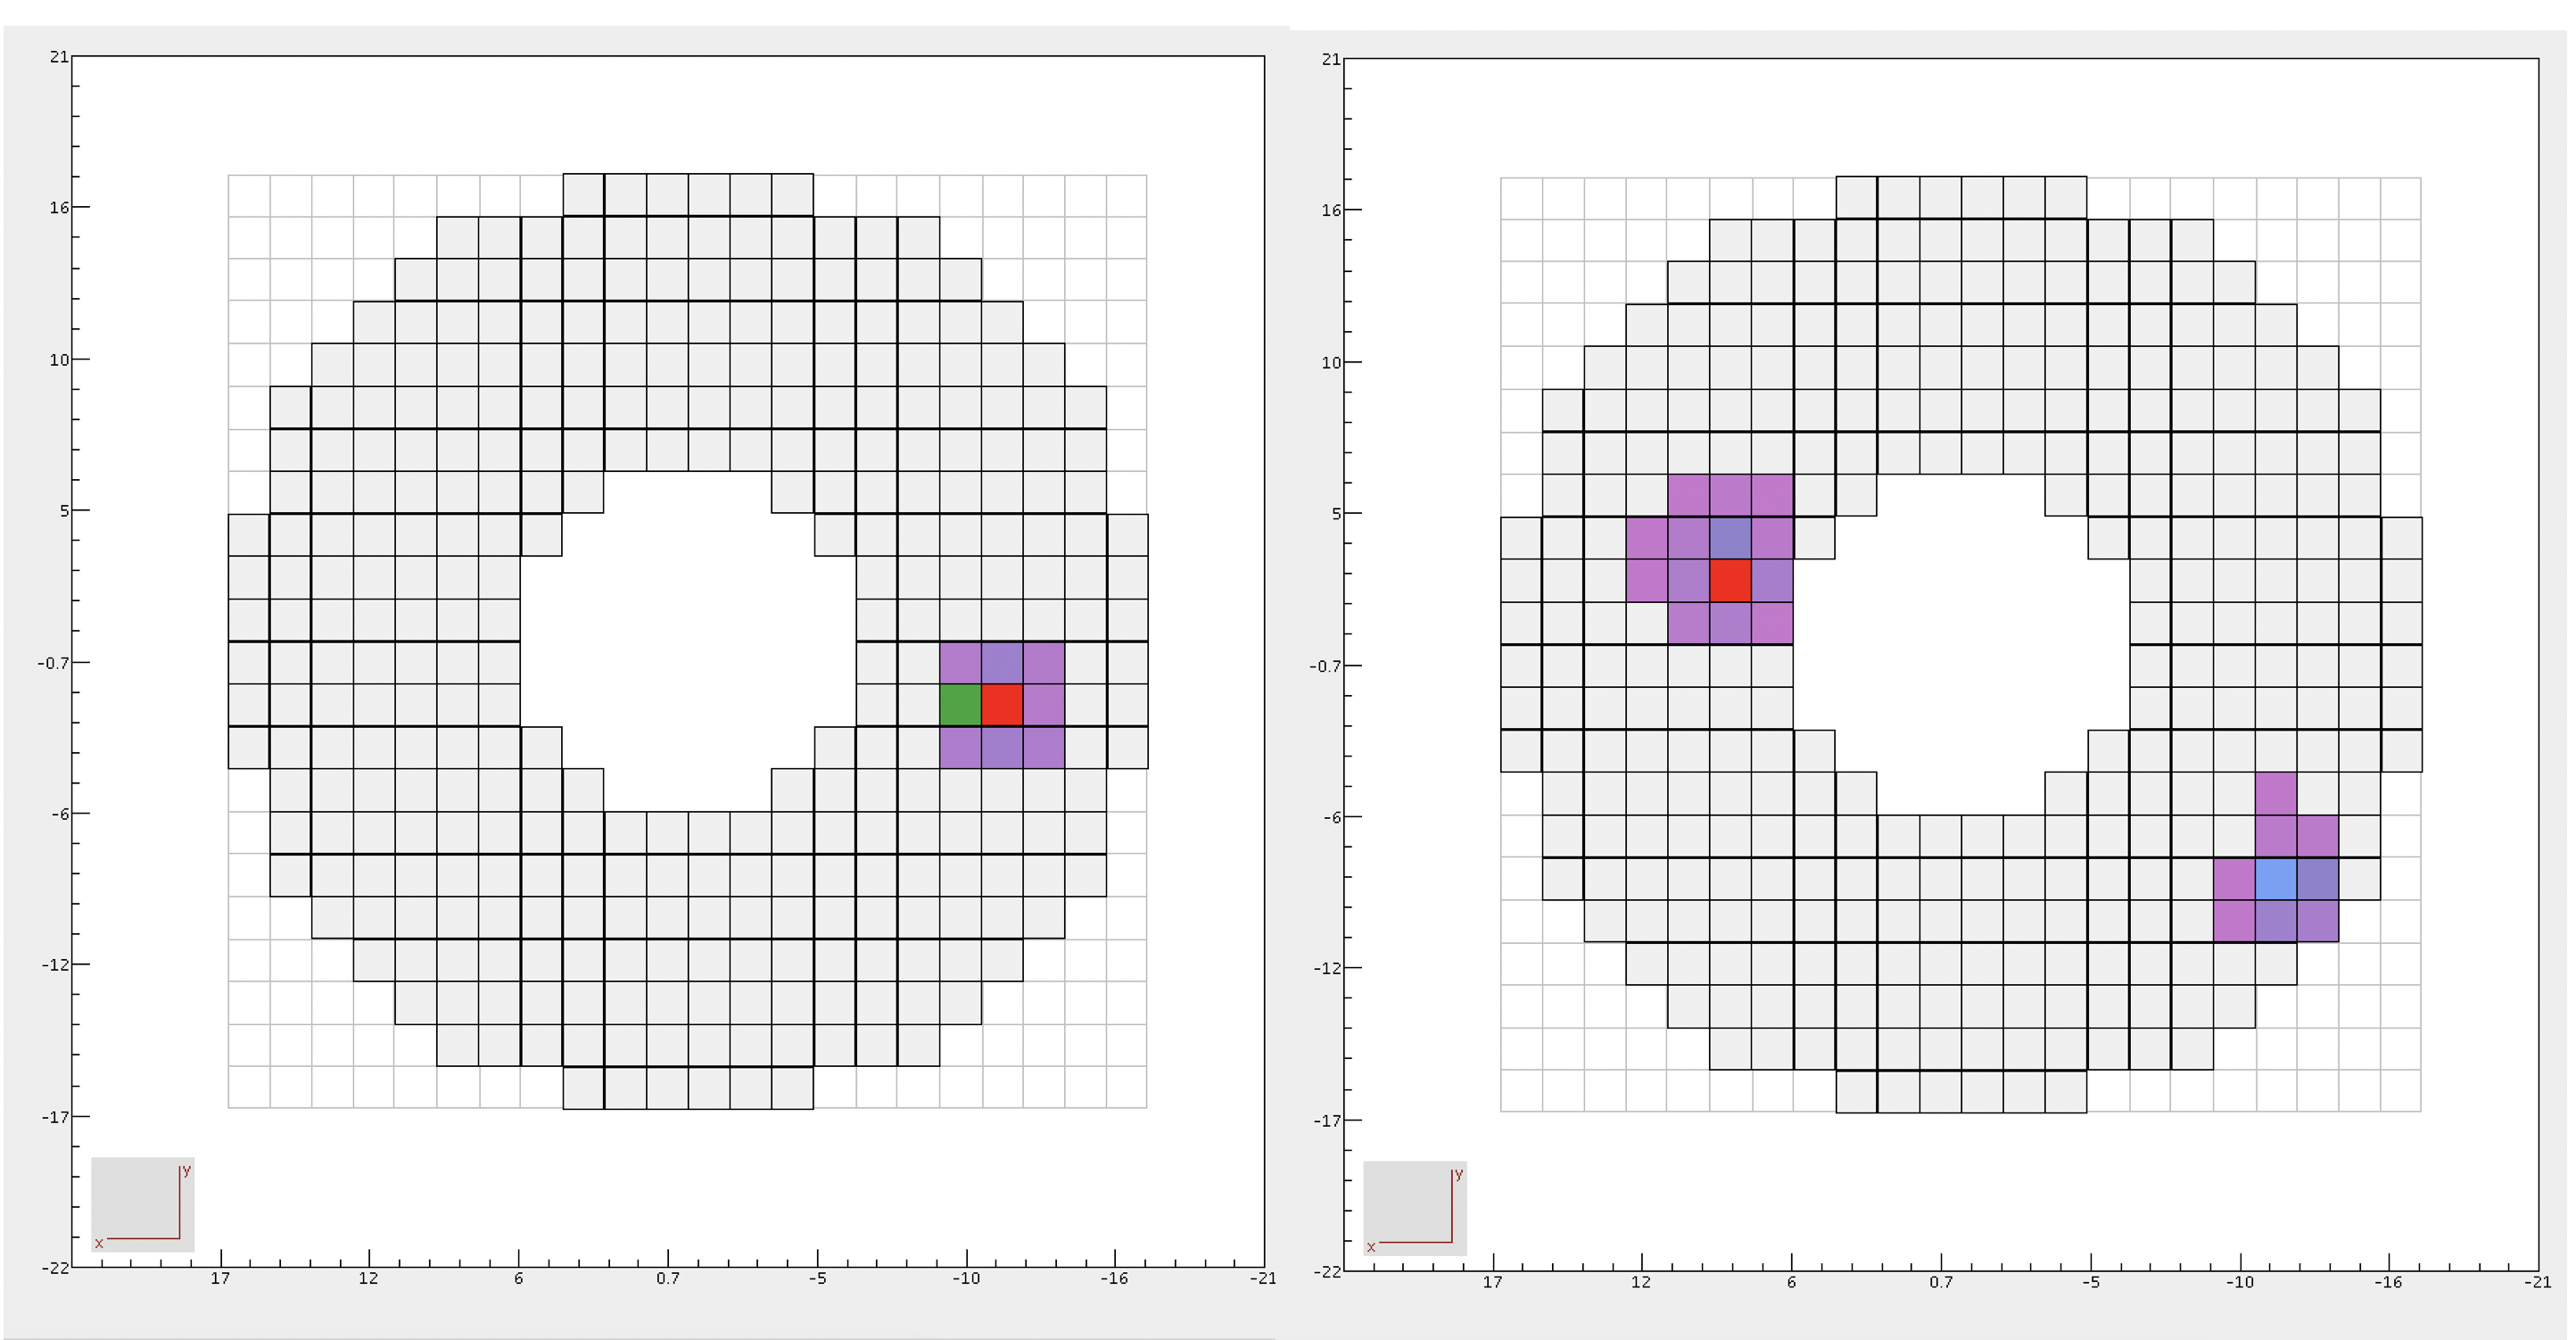
\includegraphics[width=0.95\columnwidth,keepaspectratio]{img/FT_trigger.png}
 	\caption{Display of two events selected by the Forward Tagger trigger with one and two clusters in the
          FT-Cal.}
	\label{fig:FT_trigger}
\end{figure}

The trigger configuration 
 \begin{align*} 
 &FT(E^{FT}_{min}{<}E{<}E^{FT}_{max})\times FTHodo(2)\times\\
 & [FTOF(E{>}E^{FTOF}_{min})\times PCAL(E{>}E^{PCAL}_{min})\times  DC]_i
\end{align*}
was used in the first CLAS12 experiments to select the reaction 
$$ep\to e'h^{+/-}_F X$$
with at least one electron and one particle $h^{+/-}_F$ with a definite charge in the final state. The charge of
the particle is a trigger parameter. The trigger can select negative, positive, or a particle with any charge in
the final state. $FTHodo(2)$ denotes the inclusion of the hodoscope in the trigger with hits in both planes,
correlated in space with a FT-Cal cluster. The index $i$ denotes the CLAS12 sector number. Each detector
has its own trigger energy cuts: $ E^{FT}_{min}$,  $E^{FT}_{max}$, $E^{FTOF}_{min}$, and $E^{PCAL}_{min}$. A space
correlation matching requirement between the FTOF and PCAL elements was implemented. The DAQ bandwidth
limitations require prescaling of this trigger.

The selection of the events with at least one electron and two charged particles in the forward direction
detected in different sectors
$$
ep\to e' h^{+/-}_F h^{+/-}_F X
$$ 
was done by the trigger configuration
 \begin{align*} 
 &FT(E^{FT}_{min}{<}E{<}E^{FT}_{max}) \times FTHodo(2)\times\\
 & [FTOF(E{>}E^{FTOF}_{min})\times  PCAL(E{>}E^{PCAL}_{min})\times   DC]_i \times \\
 & [FTOF(E{>}E^{FTOF}_{min})\times  PCAL(E{>}E^{PCAL}_{min})\times   DC]_j,
\end{align*}
where $i$ and $j$ denote different CLAS12 sectors. 
 
The central detectors, such as Central Time-of-Flight (CTOF) and Central Neutral Detector (CND), were used
for the selection of the events with at least one  particle detected in the Central Detector. The trigger
configuration
 \begin{align*} 
 &FT(E^{FT}_{min}{<}E{<}E^{FT}_{max}) \times FTHodo(2)\times\\
 & [FTOF(E{>}E^{FTOF}_{min})\times  PCAL(E{>}E^{PCAL}_{min})\times   DC]_i \times \\
 & CTOF(E{>}E^{CTOF}_{min})\end{align*}
\noindent
was used for the selection of events with an electron in the FT, at least one charged particle going in the forward
direction, and at least one particle detected in the central detectors. 
$$
ep\to e' h^{+/-}_F  h^{+/-}_C X.
$$
Here $h^{+/-}_C$ stands for the charged particle in the Central Detector.

The CND detector could be  added to the coincidence chain with a space correlation between the CTOF and
CND counters in case the trigger rate is too high
 \begin{align*} 
 &FT(E^{FT}_{min}{<}E{<}E^{FT}_{max})\times FTHodo(2)\times \\
 & [FTOF(E{>}E^{FTOF}_{min})\times  PCAL(E{>}E^{PCAL}_{min})\times   DC]_i \times \\
 & CTOF(E{>}E^{CTOF}_{min})\times  CND(E{>}E^{CND}_{min}).
\end{align*}
\noindent
As stated above, the minimum energy depositions in all detectors in the trigger are parameters that depend
on the individual experiment requirements.

\subsection{$J/\psi$ Meson Trigger}
\label{sec:meson_trigger}

A special trigger was designed to detect the quasi-photoproduction of $J/\psi$-mesons
$$
ep \to e' p' J/\psi, ~~~J/\psi \to \mu^+\mu^-.
$$
Two decay modes are useful for the selection of the $J/\psi$ meson: $J/\psi \to e^+e^-$ and
$J/\psi \to \mu^+\mu^-$. The conventional electron and photoproduction triggers  select the $J/\psi$-meson
in case of its decay to an electron-positron pair. However, these trigger configurations do not work with
muons in the final state. Therefore, another trigger was added to select one more decay mode for this
experiment. The CLAS12 spectrometer has no dedicated muon system, but it turns out that the selection of
particles with energy deposition in the PCAL-EC calorimeters close to the minimum-ionizing  value is sufficient
to suppress the background from pions when the invariant mass of the two particles (muons or pions) is near the
$J/\psi$-mass. The muons from the $J/\psi$ decay appear in opposite CLAS12 sectors, which allowed for the
trigger configuration:  
\begin{align*} 
 & [FTOF(E{{>}}5){\times}  PCAL(15{<}E{<}60){\times} \\
 & {\qquad} EC(60{<}E{<}120){\times}   DC]_i {\times} \\
 & [FTOF(E{{>}}5){\times}  PCAL(15{<}E{<}60){\times} \\
 & {\qquad} EC(60{<}E{<}120){\times}   DC]_j  .
\end{align*}
\noindent
The energy units are in MeV. Note, that there is no requirement to search for the scattered electron at all. This
gives an order of magnitude advantage in the  virtual photon flux in comparison with the case when the electron
is detected in the FT calorimeter. The event display with two particles with opposite charges and in the opposite
sectors, selected by the muon trigger, is shown in Fig.~\ref{fig:muon}.

\begin{figure}[!htb]
 	\centering
  	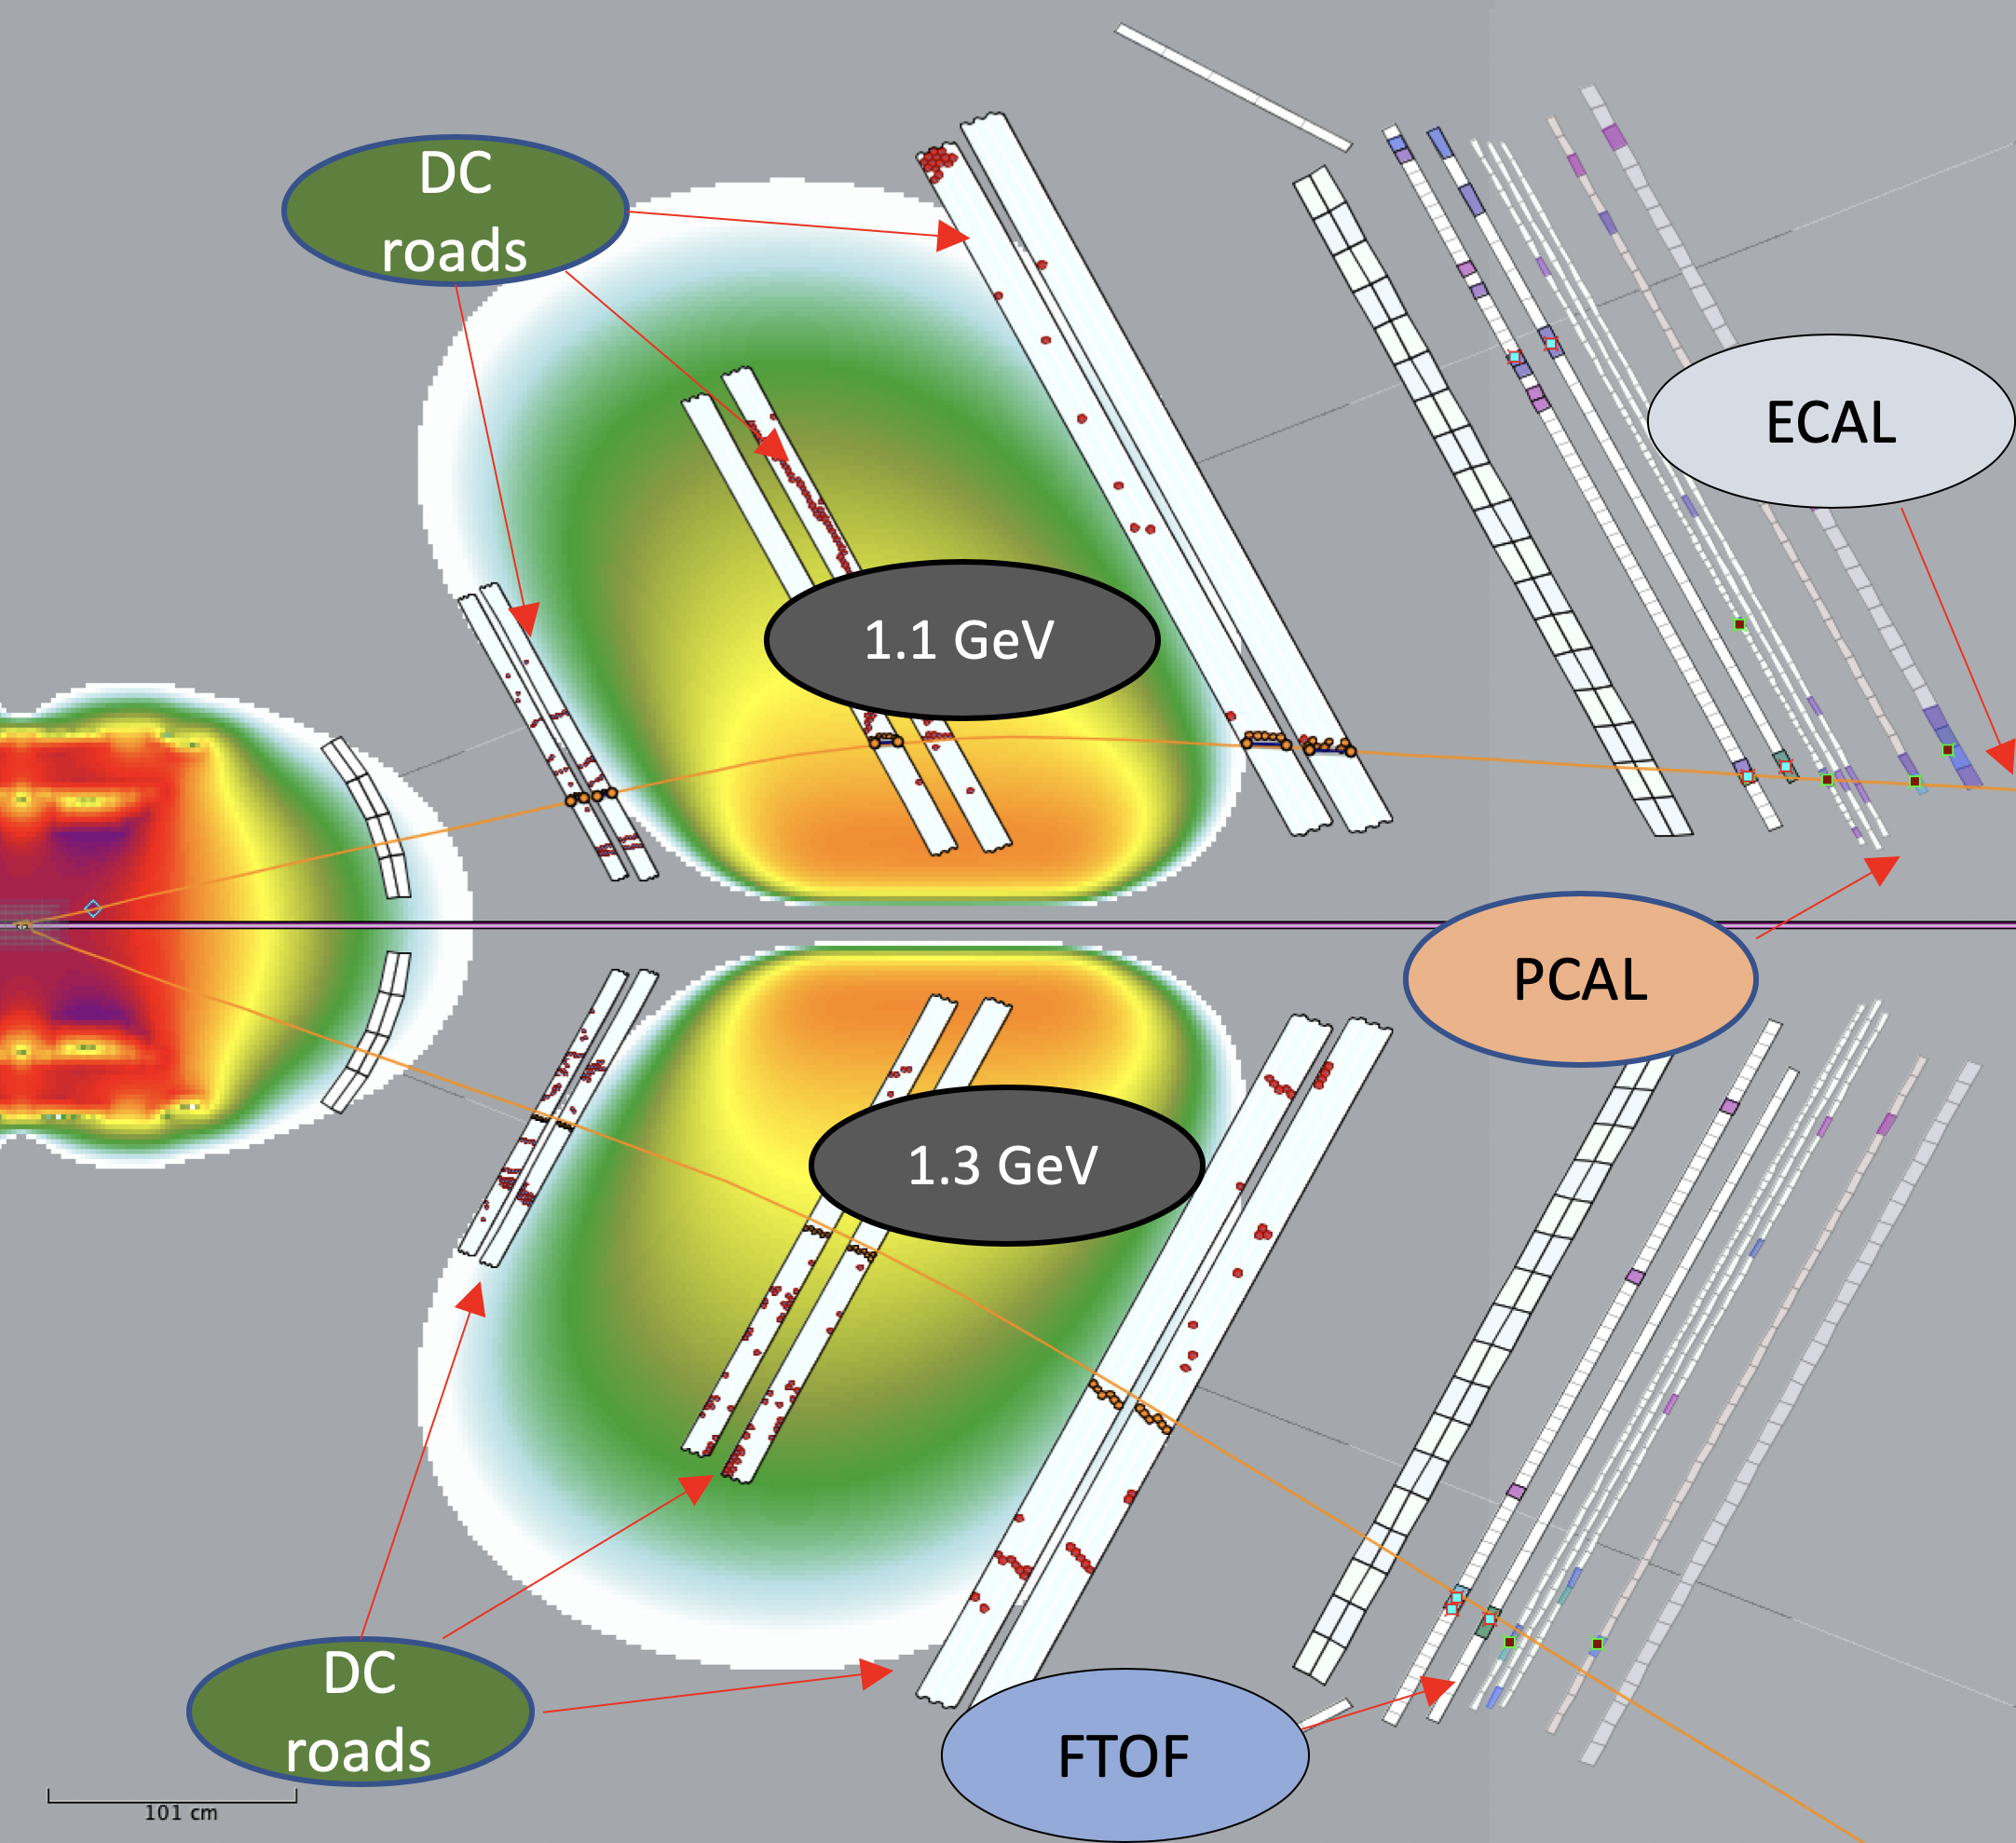
\includegraphics[width=0.95\columnwidth,keepaspectratio]{img/Muon_trigger.png}
 	\caption{CLAS12 event display of an event selected by the muon trigger. The trigger detectors DC, FTOF,
          PCAL, and EC are indicated. The particle momenta are 1.1 and 1.3~GeV.}
	\label{fig:muon}
\end{figure}
\noindent



